\section{Хөгжүүлсэн байдал}
Чатбот системийн хөгжүүлэлтийг хийхдээ шаардлагууд дээр үндэслэн, үечилсэн төлөвлөгөө болон шаардлагатай хөгжүүлэлтийг дэс дараалалтайгаар хийж гүйцэтгэсэн.
\begin{itemize}
  \item Өгөгдөл цуглуулах
  \item Өгөгдлийг нэгтгэх, цэвэрлэх
  \item Системийн шаардлага, үйл ажиллагааг тодорхойлох
  \item Өгөгдөлд анализ хийх
  \item Эх хэлний боловсруулалт хийх
  \item Чатбот хөгжүүлэх
\end{itemize}
гэсэн дарааллын дагуу хөгжүүлэлтийг хийсэн болно.
\begin{figure}[ht]
  \centering
  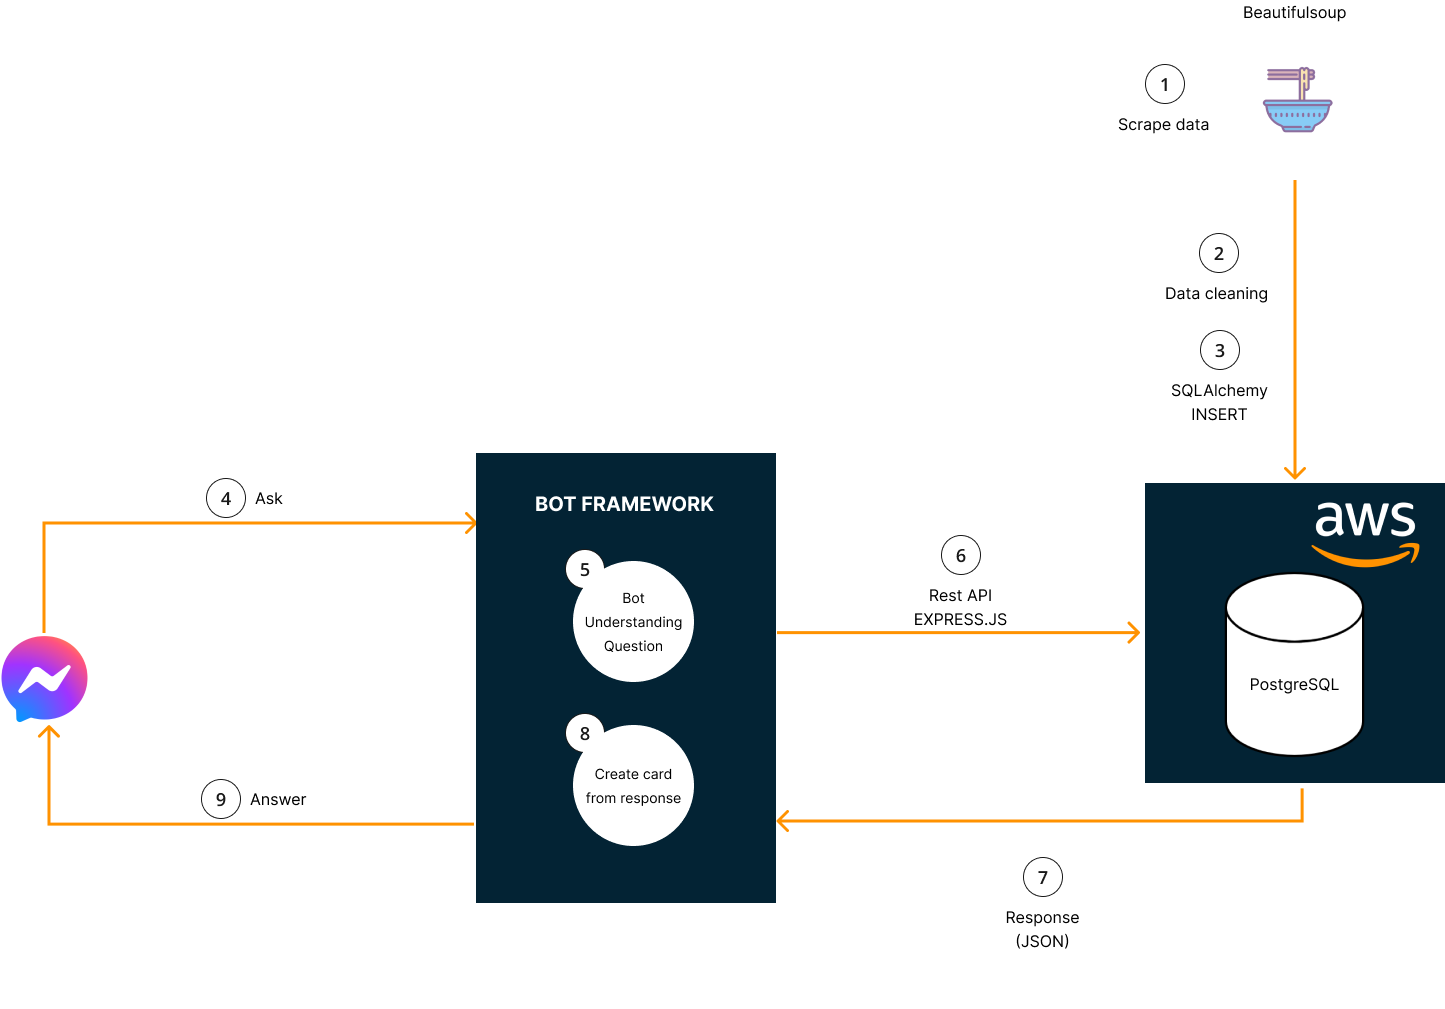
\includegraphics[width = \textwidth]{images/mainProcess.png}
  \caption{Үндсэн процесс зураглал}
\end{figure}
\\Доорх зурагт чатбот системийн үндсэн процессийн зураглал харагдаж байна. 

\newpage
\subsection{Өгөгдөл цуглуулах}
Үндсэн ашиглагдах өгөгдөл болох ажил олгогчид, ажлын байрны өгөгдлийг \textbf{zangia.mn}-ээс BeautifulSoup ашиглан авсан. Эхлээд вебсайтынхаа HTML бүтцийг нь судалж, авах өгөгдлийнхөө класс утгуудыг (className) олж авах нь зөв юм. Вебсайтаас өгөгдөл цуглуулах 2 үндсэн арга байдгаас өгөгдлийг олж илрүүлж, хаягийг цуглуулах (data crawling) аргаар бүх ангиллуудын хаяг (url)-уудын түүж авна. Харин data scraping нь тэр хооронд олсон бүх хаягуудаараа явж хэрэгтэй агуулгыг цуглуулна. \footnote{Кодын жишээг оруулахад utf-8 формат танихгүй байсан тул монголоос галиглаж бичсэн болно.}
\lstinputlisting[language=Python, firstline=9, lastline=39, caption=Data Link crawling]{code/dataScrapping.py}
Дээрх код нь эхлээд вебсайтруу орж ``filter'' класс доторх ``Салбар, мэргэжил'' гэсэн хэсгээс бүх эцэг категориудыг data crawling хийж авч байна. Үүний дараа хүүхэд категориудыг олж categorySet дотор бүх хаягуудыг хийж хадгалж байна. \footnote{Python хэлний set өгөгдлийн төрөл нь давхацахгүй утгуудын хүснэгт гэж хэлж болно. } Энд categorySet set-ийн элемент нь category төрлийн объект бөгөөд өгөгдлийн сангийн диаграм дээр тодорхойлж өгсөн байгаа. Ингэснээр data crawling-ийг зогсоож, цуглуулсан хаягаасаа өгөгдлөө цуглуулъя.  
\lstinputlisting[language=Python, firstline=41, lastline=59, caption=Өгөгдөл цуглуулах]{code/dataScrapping.py}
Дээрх кодонд бүх хүүхэд категориудын дотор агуулагдаж буй зарын мэдээллийг цуглуулж байна. Ингэхдээ эхлээд категори доторх өгөгдлүүд нь хуудаслагдсан (pagination) байх боломжтой бөгөөд хэрэв олон хуудастай байвал хаягуудыг нь угсарч тэдгээрээс ч мөн өгөгдлийг нь цуглуулах ёстой юм. 
\lstinputlisting[language=Python, firstline=3, caption=Хуудаслалтыг задлах]{code/pagination.py}
Энэ хэсэгт хуудаслан дугаарласан хэсгийн хамгийн сүүлийн тоог авч \textit{createLinkList} функцруу дамжуулснаар тухайн категорийн бүх өгөгдлийг цуглуулах боломж үүсч байгаа юм. Ингээд дахин data crawling хийж бүх хаягуудыг цуглуулж энэ удаад dictionary үүсгэж зарын хаягуудыг хадгалсан. Энд disctionary үүсгэхдээ хаягийг нь түлхүүр (key) болгож категори объектыг нь утга(value) болгож хадгалсан. Мэдээж хэрэг dictionary нь түлхүүр давхцахаас сэргийлдэг тул бид ямар нэгэн байдлаар нэг зарын өгөгдлийг 2 удаа цуглуулах эрсдэлгүй болж байна. \footnote{Нэг зарын өгөгдлийг цуглуулахад интернетийн хурдаас хамааран 0.2-оос 0.5 секунтын хугацаа зарцуулдаг}

Харин одоо үүсгэсэн dictionary-оо ашиглан өгөгдлөө CSV файлруугаа бичихэд ашиглаж болно. 
\lstinputlisting[language=Python, firstline=60, lastline=109, caption=CSV файлруу хадгалах]{code/dataScrapping.py}
Дээрх код нь энгийн python програм файлтай харьцаж өөрт цуглуулсан өгөгдлөө хадгалж байна. Нийт өгөгдлийн хүснэгтийг энд \footnote{\url{https://docs.google.com/spreadsheets/d/1rtATUKhUlleIKaWgFGvqiUWMipsrv-aCWZk-tYmzezU/edit?usp=sharing}} оруулав.

\begin{figure}[ht]
  \centering
  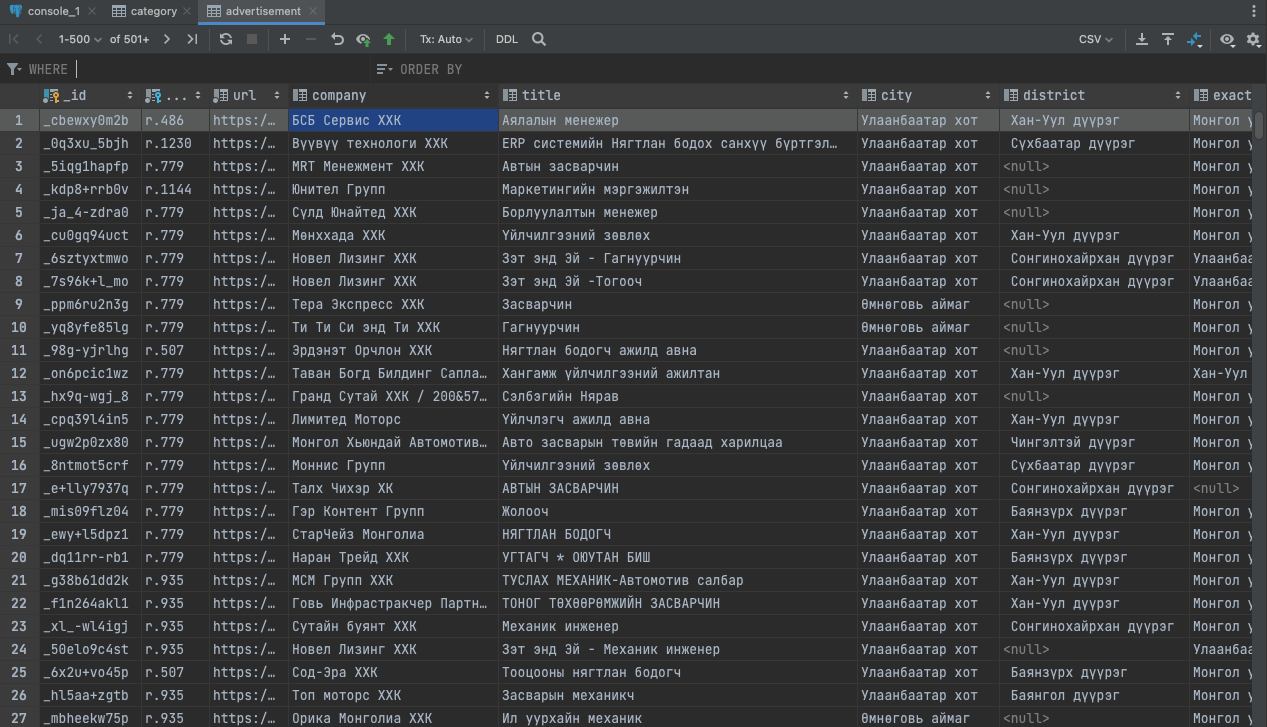
\includegraphics[width=\textwidth]{images/dataSet.png}
  \caption{Data set}
  \label{fig:dataSet}
\end{figure}
Энд хамгийн сүүлд буюу 3 сарын 31нд өгөгдлийн цуглуулга хийж 9175 өгөгдлийн excel хэлбэрт оруулсныг харж болж байна. 
\subsection{Өгөгдлийг нэгтгэх, цэвэрлэх}
Ихэнх цуглуулсан өгөгдөл нь өгөгдлийн сангийн диаграмын дагуу амжилттай цуглуулсан бөгөөд дүн шинжилгээ хийх боломжтой өгөгдлүүдийг тусад нь хадгалж ашигласан болно. 